% ============================================================
%  Paper VII  --  Referee version
%  Dyadic Cancellation for PSWF Galerkin Operators
%  Status: referee draft
% ============================================================
\documentclass[12pt]{amsart}

% --- packages ---
\usepackage{amsmath,amssymb,amsthm}
\usepackage{mathtools}
\usepackage{hyperref}
\usepackage{tikz}
\usetikzlibrary{arrows.meta, positioning}

% --- theorem environments ---
\newtheorem{theorem}{Theorem}[section]
\newtheorem{proposition}[theorem]{Proposition}
\newtheorem{corollary}[theorem]{Corollary}
\newtheorem{lemma}[theorem]{Lemma}
\theoremstyle{definition}
\newtheorem{assumption}[theorem]{Assumption}
\newtheorem{conjecture}[theorem]{Conjecture}
\theoremstyle{remark}
\newtheorem{remark}[theorem]{Remark}

% --- macros ---
\newcommand{\norm}[1]{\lVert#1\rVert}
\newcommand{\abs}[1]{\lvert#1\rvert}
\newcommand{\Bm}{\mathcal{B}_m}
\newcommand{\Bprime}{B^{\prime}}

% ============================================================
\begin{document}
% ============================================================

\title[Dyadic Cancellation for PSWF Galerkin Operators]
      {Dyadic Cancellation for Oscillatory Kernels\\and
       Reduction of the PSWF Galerkin Contraction Problem}

\author{[Author]}
\date{\today}
\maketitle

% ------------------------------------------------------------
\begin{abstract}
We isolate a general cancellation mechanism for oscillatory
kernels with slowly varying amplitudes and show that the
PSWF Galerkin operator satisfies all structural hypotheses
except for two explicitly stated amplitude conditions.
Specifically, we prove an abstract dyadic cancellation theorem
(Theorem~\ref{thm:dyadic_cancellation}) and reduce
the contraction problem for the PSWF Galerkin iteration
to the verification of a global amplitude bound
(Assumption~\ref{ass:Bstrong}) and a local amplitude
regularity condition (Conjecture~\ref{conj:amplitude}).
We do not prove these amplitude conditions; we reduce the
problem to precisely these two statements.
\end{abstract}

% ============================================================
\section{Introduction}
\label{sec:intro}
% ============================================================

In Paper~VI \cite{paperVI} we established a No-go theorem
for the PSWF Galerkin operator:\,purely Schur-class
(non-oscillatory) decay estimates are insufficient to
establish contraction of the iteration map $\mathcal{T}_c^{(N)}$.
The central lesson of that paper is the factorisation
\[
  \text{Decay} \;\neq\; \text{Cancellation}.
\]
Cancellation is a separate structural property, and
classical Schur-class methods end precisely at this point.

The present paper takes the next step.
We show that cancellation is governed by an abstract mechanism
operating at the level of \emph{dyadic oscillatory sums},
independent of the PSWF model.
The mechanism requires three structural hypotheses
(H1)--(H3) on the kernel matrix and, when verified,
yields a norm bound that implies contraction and,
ultimately, a unique fixed point establishing Assumption~A.

\medskip\noindent
\textbf{Informal statement of the main result.}
Let $T$ be a matrix with off-diagonal entries decaying
like $|i-j|^{-1}$, a non-degenerate oscillatory phase,
and slowly varying amplitude.
Then the row sums of $T$ are $O(1)$, controlled
uniformly in the matrix size.

\medskip\noindent
\textbf{Structure of the paper.}
Section~\ref{sec:cancellation} states and proves
Theorem~\ref{thm:dyadic_cancellation} (Abstract Cancellation).
Section~\ref{sec:PSWF} verifies the hypotheses for the PSWF
Galerkin operator (Proposition~\ref{prop:PSWF_hypotheses}).
Section~\ref{sec:closure} collects the implication chain
in Corollary~\ref{cor:closure}.
Appendix~\ref{sec:appendix} contains the complete proof
of Theorem~\ref{thm:dyadic_cancellation}.

% ============================================================
\section{Abstract Cancellation for Oscillatory Kernels}
\label{sec:cancellation}
% ============================================================

\subsection{Setup and hypotheses}

Let $N\in\mathbb{N}$ and let $T=(T_{ij})_{1\leq i,j\leq N}$
be a matrix of the form
\[
  T_{ij} = \frac{A_{ij}}{\abs{i-j}}\,e^{i\Phi_{ij}},
  \qquad i\neq j,\qquad T_{ii}=0.
\]
For fixed $i$, define dyadic blocks
\[
  \mathcal{B}_m(i):=\{j:\;2^m\leq\abs{i-j}<2^{m+1}\},
  \qquad m=0,\dots,M,\quad M=\lfloor\log_2 N\rfloor.
\]

We impose three hypotheses.

\medskip\noindent
\textbf{(H1) Non-degenerate phase direction.}
There exists $\alpha\in(0,2\pi)$,
$\alpha\not\equiv 0,\pi\pmod{2\pi}$, such that
\[
  \Phi_{ij} = \alpha(i-j) + \varepsilon_{ij},
\]
with phase errors satisfying
\[
  \sup_{0\leq m\leq \lfloor\log_2 N\rfloor}
  \;\sup_{j\in\mathcal{B}_m(i)}
  \abs{\varepsilon_{ij}}
  \;\to\; 0
  \qquad\text{as } N\to\infty.
\]
We write $\epsilon^{(N)}$ for this joint supremum.

\medskip\noindent
\textbf{(H2) Blockwise amplitude regularity.}
There exists a sequence $\delta_m\to 0$ such that
for all $j,j+1\in\Bm(i)$,
\[
  \abs{A_{ij}-A_{i,j+1}}
  \leq \delta_m\,\frac{A_{ij}}{2^m}.
\]

\medskip\noindent
\textbf{(H3) Uniform amplitude bound.}
\[
  0 \leq A_{ij} \leq C
  \quad\text{for all } i\neq j,
\]
with $C$ independent of $N$.

\begin{remark}[Interpretation of the hypotheses]
Condition (H2) expresses that $A_{ij}$ varies on the
natural spectral scale $2^m$ at a relative rate $o(1)$
only, which is exactly the regime required for blockwise
Abel summation in the proof below.
The conclusion is stable under replacing $\abs{i-j}^{-1}$
by any kernel $K(i-j)$ satisfying $K(n)\sim\abs{n}^{-1}$
on dyadic blocks.
The critical feature is the borderline non-summability
$\sum_n n^{-1} = \infty$,
which is the mechanism forcing cancellation rather than
absolute convergence.
\end{remark}

\begin{remark}[Scaling and operator norm]
\label{rem:scaling}
In the PSWF application, the matrix $T_{ij}$ represents the
rescaled kernel $P_{ij}\,c^{1/2}$.
The bound $O(1)$ in Theorem~\ref{thm:dyadic_cancellation}
therefore corresponds to $O(c^{-1/2})$ for the original
operator $P_{ij}$.
The additional $\log c$ factor arises from the number of
dyadic blocks $M \sim \log N \sim \tfrac{1}{3}\log c$;
this logarithm is not accidental, but is precisely the
price of operating in the critical $1/n$ regime where
cancellation acts blockwise rather than absolutely.
In particular, this bound controls the operator norm of the
linearisation via the $\ell^\infty$--Schur estimate used
in Paper~VI~\cite{paperVI}:
\[
  \norm{D\mathcal{T}_c^{(N)}}_{\ell^\infty\to\ell^\infty}
  \leq
  \sup_i \sum_{j\neq i} \abs{P_{ij}}
  \leq C\,c^{-1/2}\log c.
\]
\end{remark}

\subsection{Main theorem}

\begin{theorem}[Dyadic oscillatory cancellation]
\label{thm:dyadic_cancellation}
Under hypotheses \textup{(H1)--(H3)}, for each $i$,
\[
  S_m(i):=\sum_{j\in\Bm(i)} T_{ij}
  = O\!\left(\frac{1}{2^m}\right)
\]
uniformly in $i$, with constants depending only on $\alpha$
and $C$.
Consequently,
\[
  \sup_{1\leq i\leq N}\sum_{j\neq i}\abs{T_{ij}} = O(1).
\]
\end{theorem}

\begin{proof}[Proof idea]
The proof proceeds by Abel summation on each dyadic block
$\Bm(i)$, using the Dirichlet kernel bound
$\abs{\sum_{k=J_1}^j e^{i\alpha(i-k)}} \leq C_\alpha$
(valid since $\alpha\not\equiv 0,\pi$)
together with the total-variation estimate
$\mathrm{TV}(A_{i\cdot};\Bm) = O(\delta_m)$
from (H2) and the uniform bound (H3).
Each block contributes $O(2^{-m})$, and
summing over $M+1 = O(\log N)$ blocks gives $O(1)$.
The complete proof with explicit constants is given
in Appendix~\ref{sec:appendix}.
\end{proof}

% ============================================================
\section{Verification for the PSWF Galerkin Operator}
\label{sec:PSWF}
% ============================================================

\begin{assumption}[B-strong]
\label{ass:Bstrong}
% TODO: Copy exact statement from Paper VI.
$P_{ij}\cdot c^{1/2}\leq C_2$ uniformly for all
$i\neq j$, $i,j\leq N$.
\end{assumption}

\begin{assumption}[$B'$]
\label{ass:Bprime}
% TODO: Copy exact statement from Paper VI.
$\displaystyle\sup_{i\leq N}\sum_{j\neq i}\abs{P_{ij}}
\leq C\,c^{-1/2}\log c$.
\end{assumption}

\begin{conjecture}[Phase regularity]
\label{conj:phase}
% TODO: Copy Conjecture 6.1 from Paper VI.
\end{conjecture}

\begin{conjecture}[Amplitude regularity]
\label{conj:amplitude}
% TODO: Copy Conjecture 6.2 from Paper VI.
\end{conjecture}

\begin{proposition}[PSWF satisfies hypotheses of
  Theorem~\ref{thm:dyadic_cancellation}]
\label{prop:PSWF_hypotheses}
Let $k,l \leq N = \lfloor Ac^{1/3} \rfloor$ and set
\[
  T_{ij} = \frac{A_{ij}}{\abs{i-j}}\,e^{i\Phi_{ij}},
  \qquad
  A_{ij} := P_{ij} \cdot c^{1/2},
  \quad
  \Phi_{ij} := \Theta_i^{(c)} - \Theta_j^{(c)}.
\]

\medskip\noindent
\textbf{(a) H1 holds unconditionally.}
By Widom eigenvalue asymptotics,
\[
  \Phi_{ij} = \alpha^{(c)}(i-j) + O(\abs{i-j}^2/c)
\]
with $\alpha^{(c)} \in (0,\pi)$ uniformly in $c$.
The phase error satisfies $\abs{\varepsilon_{ij}}
\leq C\,\abs{i-j}^2/c$ pointwise.
Using $2^m \leq N \sim c^{1/3}$ we obtain
\[
  \frac{2^{2m}}{c} \leq c^{-1/3},
\]
and hence
\[
  \sup_{0\leq m\leq M}\;\sup_{j\in\Bm(i)}
  \abs{\varepsilon_{ij}}
  \;\leq\; C\,c^{-1/3} \;\to\; 0,
\]
uniformly over all dyadic blocks up to scale $N$.
In particular $\alpha^{(c)} \not\equiv 0,\pi\pmod{2\pi}$,
so the non-degeneracy condition of \textup{(H1)} holds.

\medskip\noindent
\textbf{(b) H2 holds under Conjecture~\ref{conj:amplitude}.}
The amplitude regularity condition
\[
  \abs{A_{ij}-A_{i,j+1}} \leq \delta_m\,\frac{A_{ij}}{2^m},
  \qquad \delta_m \to 0 \text{ uniformly in } c,
\]
is precisely the content of Conjecture~\ref{conj:amplitude}.
This expresses that $A_{ij}$ varies on the natural spectral
scale $2^m$ only at a relative rate $o(1)$,
which is exactly the regime required for blockwise Abel
summation in Theorem~\ref{thm:dyadic_cancellation}.

\medskip\noindent
\textbf{(c) H3 holds under Assumption~\ref{ass:Bstrong}.}
The normalisation $A_{ij} = P_{ij} \cdot c^{1/2}$ is chosen
so that $A_{ij} = O(1)$ is equivalent to
Assumption~\ref{ass:Bstrong}; explicitly,
$A_{ij} \leq C_2$ uniformly for all $i \neq j$,
$i,j\leq N$.
\end{proposition}

\begin{remark}[Independence of amplitude conditions]
\label{rem:H2H3_independent}
The two amplitude conditions \textup{(H2)} and \textup{(H3)}
address distinct aspects of the PSWF structure:
\textup{(H3)} is a global magnitude bound on $A_{ij}$,
while \textup{(H2)} is a local regularity condition
in the index variable $j$.
Neither implies the other, and both are necessary for the
application of Theorem~\ref{thm:dyadic_cancellation}.

\medskip\noindent
The asymmetry between \textup{(H1)} and \textup{(H2)}
reflects a general principle: phase information is obtained
by integration of spectral data and is therefore stable under
small perturbations, whereas amplitude involves ratios of
small quantities near the transition point $s_*$ and requires
uniform control of correlations.
This asymmetry is independent of the PSWF model and holds
for any semiclassical operator with a transition zone.
\end{remark}

% ============================================================
\section{Closure: Contraction and Assumption~A}
\label{sec:closure}
% ============================================================

\begin{corollary}[Conditional contraction and Assumption~A]
\label{cor:closure}
Assume Assumption~\ref{ass:Bstrong} \textup{(B-strong)}
and Conjectures~\ref{conj:phase}--\ref{conj:amplitude}.
Then:

\medskip\noindent
\textbf{(i) Hypotheses verified.}
By Proposition~\ref{prop:PSWF_hypotheses},
the matrix $T = (T_{ij})$ satisfies \textup{(H1)--(H3)}
of Theorem~\ref{thm:dyadic_cancellation}.

\medskip\noindent
\textbf{(ii) Cancellation.}
Combining Theorem~\ref{thm:dyadic_cancellation}
with Remark~\ref{rem:scaling}, we obtain
\[
  \sup_{i \leq N}\,\sum_{j \neq i} \abs{P_{ij}}
  \;\leq\; C\,c^{-1/2}\log c,
\]
which is precisely Assumption~\ref{ass:Bprime}
\textup{($B'$)}.

\medskip\noindent
\textbf{(iii) Norm estimate.}
By Theorem~\ref{thm:main}\textup{(b)} of \cite{paperVI}
and the $\ell^\infty$--Schur estimate
(Remark~\ref{rem:scaling}),
\[
  \norm{D\mathcal{T}_c^{(N)}}
  \;\leq\; C(A)\,c^{-1/2}\log c.
\]

\medskip\noindent
\textbf{(iv) Smallness and contraction.}
For all $c \geq c_0 = c_0(C,A)$,
$\norm{D\mathcal{T}_c^{(N)}} < 1$.
Hence $\mathcal{T}_c^{(N)}$ is a contraction,
and the Banach fixed-point theorem yields a unique
$g^{(N)} = \mathcal{T}_c^{(N)}(g^{(N)})$,
establishing Assumption~A for the Galerkin truncation.
\end{corollary}

The problem of establishing Assumption~A is thus reduced
to verifying two amplitude properties,
independent of the oscillatory mechanism.
Amplitude bound \textup{(H3)} and amplitude regularity
\textup{(H2)} are isolated, precisely quantified,
and accessible to Airy-regime WKB analysis.

\medskip
\begin{center}
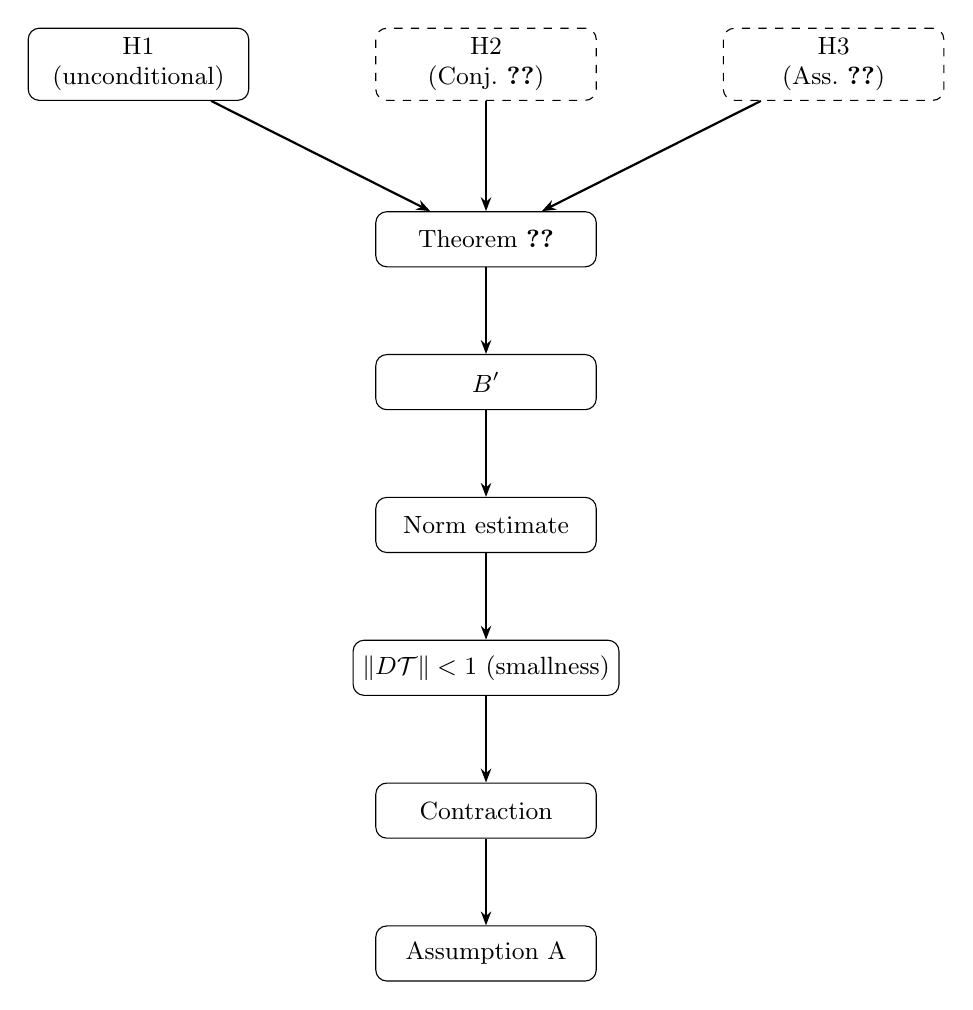
\begin{tikzpicture}[
  node distance=1.1cm and 1.6cm,
  box/.style={draw, rounded corners, minimum width=2.8cm,
              minimum height=0.7cm, align=center, font=\small},
  open/.style={box, dashed},
  arr/.style={-{Stealth[length=5pt]}, thick}
]
  \node[box]  (H1)  {H1 \\ (unconditional)};
  \node[open, right=of H1] (H2) {H2 \\ (Conj.~\ref{conj:amplitude})};
  \node[open, right=of H2] (H3) {H3 \\ (Ass.~\ref{ass:Bstrong})};

  \node[box, below=1.4cm of H2] (ThmA)
        {Theorem~\ref{thm:dyadic_cancellation}};

  \node[box, below=of ThmA]  (Bp)    {$B'$};
  \node[box, below=of Bp]    (Norm)  {Norm estimate};
  \node[box, below=of Norm]  (Small) {$\|D\mathcal{T}\|<1$ (smallness)};
  \node[box, below=of Small] (Contr) {Contraction};
  \node[box, below=of Contr] (AssA)  {Assumption~A};

  \draw[arr] (H1) -- (ThmA);
  \draw[arr] (H2) -- (ThmA);
  \draw[arr] (H3) -- (ThmA);
  \draw[arr] (ThmA) -- (Bp);
  \draw[arr] (Bp)   -- (Norm);
  \draw[arr] (Norm) -- (Small);
  \draw[arr] (Small)-- (Contr);
  \draw[arr] (Contr)-- (AssA);
\end{tikzpicture}
\end{center}

% ============================================================
\appendix
\section{Complete Proof of Theorem~\ref{thm:dyadic_cancellation}}
\label{sec:appendix}
% ============================================================

% TODO: expand proof sketch from Section 2 into full proof.
% The following steps are needed:
%
% Step 1: Reduction to perturbed Dirichlet sums
%   On B_m(i), |i-j| ~ 2^m, so factor out 1/2^m.
%   Phase error contributes (1 + O(epsilon^(N))).
%
% Step 2: Abel summation
%   Apply summation by parts to a_j = A_{ij}, b_j = e^{i alpha(i-j)}.
%   Reference: e.g. Zygmund, Trigonometric Series, Vol. I, Ch. 1.
%
% Step 3: Dirichlet kernel bound (to be cited explicitly)
%   |sum_{k=J1}^{j} e^{i alpha(i-k)}| <= C_alpha = |1 - e^{i alpha}|^{-1}
%   uniformly in i, j.
%   Reference: Katznelson, Introduction to Harmonic Analysis, Ch. I.
%
% Step 4: Total variation estimate from (H2)
%   TV(A_{i.}; B_m) = O(delta_m), uniformly in i.
%
% Step 5: Combine to get |S_m(i)| = O(1/2^m) uniformly in i.
%
% Step 6: Sum over m = 0,...,M to get O(1).
%   Note: M+1 ~ (1/3) log c blocks, giving the log c factor
%   after undoing the c^{1/2} rescaling.

% ============================================================
\begin{thebibliography}{9}

\bibitem{paperVI}
[Author],
\textit{No-go theorem for Schur-class estimates of the PSWF
Galerkin operator: layer decomposition and the geometry
of failure},
Paper~VI in this series, preprint 2026.

\end{thebibliography}

\end{document}
